\documentclass[conference]{IEEEtran}

\usepackage{cite}
\usepackage{amsmath,amssymb}
\usepackage{graphicx}
\usepackage{booktabs}
\usepackage{array}
\usepackage{tabularx}
\usepackage{url}
\usepackage{tikz}
\usetikzlibrary{arrows.meta,positioning,shapes.geometric}
\usepackage[hidelinks]{hyperref}

\graphicspath{{figures/}}

\begin{document}

\title{Does Agent Disagreement Tell an LLM When to Deliberate?\\
A Frozen-Protocol Study of Demand Forecasting}

\author{\IEEEauthorblockN{[Author Name]}
\IEEEauthorblockA{[Department, University]\\
[City, Country]\\
[email]}}

\maketitle

\begin{abstract}
Calling a large language model (LLM) on every demand forecast is costly, and a natural shortcut is
to call it only when specialised forecasting agents disagree. This paper tests that idea under a
frozen protocol. In RetailSense, a LightGBM Historical agent and Calendar, Weather and Trend agents
forecast daily item demand; a confidence-weighted disagreement score $D$ triggers an LLM critic and
one bounded revision round when $D$ reaches a threshold frozen on validation data. Code, never the
LLM, computes the final forecast and the order quantity, and every system passes through one
$(s,S)$ inventory simulator. One locked test run per dataset covers a simulated Mumbai grocery store
with logged demand drivers and real sales from the Czech online grocer Rohlik. On the test splits,
disagreement is a weak risk signal (Spearman $\rho=0.072$ on simulated India, $0.119$ on real
Rohlik). Selective deliberation does not improve accuracy: it is statistically equivalent to
always-on deliberation, to random triggering and to no deliberation within 1\% of WAPE. Its only
demonstrated benefit is efficiency (73--83\% fewer LLM calls than always-on at that equivalent
accuracy), not a gain in accuracy. Stronger single models beat every multi-agent variant: an
all-features LightGBM on India (test WAPE 0.369 vs 0.378) and ETS on Rohlik (0.150 vs 0.175). No
multi-agent system has the lowest inventory cost on either dataset.
A post-hoc diagnosis shows that the failure is not an artefact of correlated agents: agents built
on independent evidence do not make $D$ a better warning for the strong forecaster, and their only
large deliberation gain repairs errors they introduce. Logged drivers show that an 8B critic partly
identifies the true driver but its revisions ignore it; a 31B critic acts on it, yet selecting cases
by $D$ remains no better than chance. In this setting, disagreement is not a reliable trigger for
LLM deliberation.
\end{abstract}

\begin{IEEEkeywords}
demand forecasting, multi-agent systems, large language models, forecast disagreement, selective
deliberation, equivalence testing, inventory control
\end{IEEEkeywords}

% =====================================================================
\section{Introduction}

A store manager who restocks shelves every week has to decide how much of each item to order
before demand is known. Ordering too little loses sales; ordering too much ties up cash and shelf
space. The forecast behind that decision draws on several kinds of evidence: recent sales, the
calendar, the weather and shifts in customer interest. Machine-learning models such as
LightGBM~\cite{ke2017} combine these signals well, and gradient-boosted models dominated the large
M5 retail benchmark~\cite{makridakis2022}. Large language models (LLMs) may add a different
ability: in principle they can read conflicting evidence and reason about which source to
trust~\cite{du2024}. Each LLM call, however, costs time and money, and the value of calling the
model on every item and every day is not obvious~\cite{tan2024}.

The closest prior system, and the base work for this paper, is MARIOD~\cite{yang2025}, which couples
a transformer demand forecaster with hierarchical multi-agent reinforcement learning and reports
lower forecast error and fewer stockouts than deep-learning and reinforcement-learning baselines.
RetailSense addresses the same problem but splits agents by \emph{evidence source} rather than by
supply-chain level, coordinates them through an explicit disagreement score and one bounded LLM
revision, and orders through a transparent $(s,S)$ policy.

The question is whether an LLM can be used \emph{selectively}, only on the forecasts where it is
most likely to help. The idea comes from forecast combination and ensemble forecasting: combining
forecasts usually beats a single forecast~\cite{bates1969,timmermann2006,wang2023}, and the spread
between forecasters is a signal of uncertainty, although an imperfect
one~\cite{zarnowitz1987,whitaker1998}. If forecasters disagree, the case may be risky, and a
closer look may be worth its cost.

\subsection{Approach}

Each RetailSense agent sees one kind of evidence (Fig.~\ref{fig:system}). A Historical agent
forecasts from lagged sales and price; Calendar, Weather and Trend agents adjust that baseline using
only their own signal. The orchestrator computes a normalised disagreement score $D$. If $D<\tau$,
the system returns the confidence-weighted consensus; if $D\ge\tau$, an LLM critic explains the
conflict and each agent receives one bounded revision, following critique-then-revise and debate
methods~\cite{du2024,madaan2023} and cost-aware LLM cascades and routers~\cite{chen2023,ong2025}.
Unlike LLM-as-forecaster methods~\cite{gruver2023,jin2024}, the LLM may only propose a confidence
multiplier and a revised value inside each agent's band; code clips both and computes the final
forecast, which feeds a periodic-review $(s,S)$ policy~\cite{silver2017}.

\begin{figure}[t]
\centering
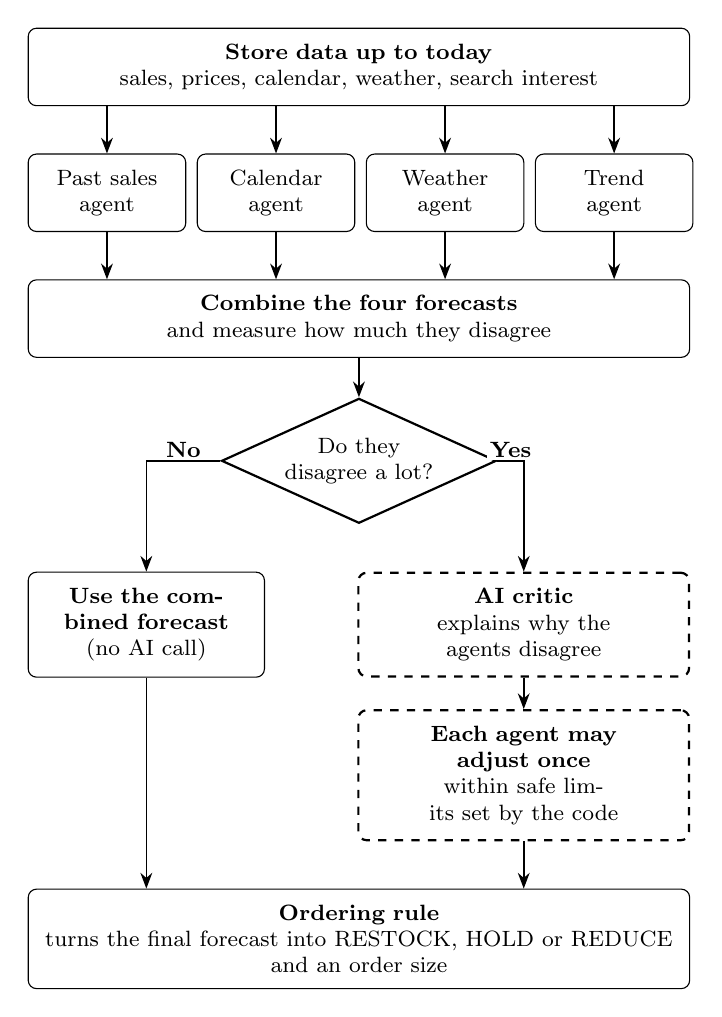
\begin{tikzpicture}[font=\footnotesize,
  box/.style={draw, rounded corners=3pt, align=center, inner sep=2mm, minimum height=8mm},
  ai/.style={box, dashed, thick},
  arr/.style={-{Stealth[length=2mm]}, semithick},
  lab/.style={font=\footnotesize\bfseries, fill=white, inner sep=1pt}]

\node[box, text width=80mm] (data) {\textbf{Store data up to today}\\
  sales, prices, calendar, weather, search interest};

\node[box, text width=16mm, anchor=north west] (a1) at ([yshift=-6mm]data.south west)
  {Past sales\\agent};
\node[box, text width=16mm, right=1.33mm of a1] (a2) {Calendar\\agent};
\node[box, text width=16mm, right=1.33mm of a2] (a3) {Weather\\agent};
\node[box, text width=16mm, right=1.33mm of a3] (a4) {Trend\\agent};

\node[box, text width=80mm, anchor=north west] (comb) at ([yshift=-6mm]a1.south west)
  {\textbf{Combine the four forecasts}\\ and measure how much they disagree};

\node[draw, diamond, aspect=2.2, align=center, inner sep=0.5mm, thick,
      below=5mm of comb] (dia) {Do they\\ disagree a lot?};

\node[box, text width=26mm, anchor=north west] (fast) at ([yshift=-6mm]comb.south west |- dia.south)
  {\textbf{Use the combined forecast}\\ (no AI call)};
\node[ai, text width=38mm, anchor=north east] (crit) at ([yshift=-6mm]comb.south east |- dia.south)
  {\textbf{AI critic}\\ explains why the agents disagree};
\node[ai, text width=38mm, below=4mm of crit] (rev)
  {\textbf{Each agent may adjust once}\\ within safe limits set by the code};

\node[box, text width=80mm, anchor=north] (order) at ([yshift=-6mm]comb.south |- rev.south)
  {\textbf{Ordering rule}\\ turns the final forecast into RESTOCK, HOLD or REDUCE\\ and an order
  size};

\foreach \a in {a1,a2,a3,a4} {
  \draw[arr] (data.south -| \a.north) -- (\a.north);
  \draw[arr] (\a.south) -- (\a.south |- comb.north);
}
\draw[arr] (comb) -- (dia);
\draw[arr] (dia.west) -| node[lab, pos=0.25, above]{No} (fast.north);
\draw[arr] (dia.east) -| node[lab, pos=0.25, above]{Yes} (crit.north);
\draw[arr] (crit) -- (rev);
\draw[arr] (fast.south) -- (fast.south |- order.north);
\draw[arr] (rev.south) -- (rev.south |- order.north);
\end{tikzpicture}
\caption{How RetailSense works. Four agents each forecast demand from one kind of information. If
they mostly agree, their combined forecast is used straight away. If they disagree a lot, an AI
critic explains the conflict and each agent may adjust its forecast once, within limits set by the
code. A fixed ordering rule, not the AI, decides how much to order. Dashed boxes are AI steps.}
\label{fig:system}
\end{figure}

\subsection{Research Question and Hypotheses}

The research question is: \emph{does disagreement-triggered deliberation among heterogeneous
forecasting agents improve demand forecasting and restocking decisions compared with statistical
forecasting, a single model, simple multi-agent consensus and always-on deliberation?} It is split
into five hypotheses:
\begin{itemize}
\item \textbf{H1.} Normalised disagreement $D$ is positively associated with forecast error.
\item \textbf{H2.} Deliberation lowers error on the cases it is triggered for.
\item \textbf{H3.} Selective deliberation matches always-on deliberation at a fraction of the LLM
cost.
\item \textbf{H4.} Disagreement is a better trigger than chance.
\item \textbf{H5.} Better forecasts translate into better inventory outcomes.
\end{itemize}
H4 is the central test: if a random trigger at the same rate does as well, the disagreement signal
adds nothing.

\subsection{Contributions}

\begin{enumerate}
\item \textbf{A frozen evaluation protocol for selective LLM use.} $\tau$ and the prompt are frozen
on validation before each dataset's single test run; every system passes through one inventory
simulator; a random trigger at the same rate isolates the value of $D$; and claims of ``no
difference'' are backed by equivalence tests~\cite{schuirmann1987} and minimum detectable effects
rather than by non-significant tests.
\item \textbf{A simulator with logged ground-truth drivers.} The primary dataset is a simulated
Indian kirana (neighbourhood grocery) chain built from real Open-Meteo weather~\cite{openmeteo} and
a real festival calendar. Every demand multiplier is logged, which makes it possible to check
whether the critic identifies the evidence that actually drove demand.
\item \textbf{A diagnosis of why selective deliberation fails.} Declared post-hoc analyses on
validation vary the agent design (residual adjusters, item-aware, fully independent evidence), the
critic (8B and 31B) and the trigger (fixed $D$, learned, random, always), and score each against the
frozen systems on the same cases. The failure survives every variant.
\item \textbf{A real-data replication with modern baselines.} The protocol is applied unchanged to
real daily sales from Rohlik, a Czech online grocer~\cite{rohlik}, and compared with a single
all-features LightGBM, ETS and a zero-shot foundation model, Chronos~\cite{ansari2024}.
\end{enumerate}

\subsection{Summary of Findings}

On both test splits, $D$ is weakly but significantly associated with error. Selective deliberation
is equivalent to always-on deliberation, to random triggering and to no deliberation within 0.5\%
of WAPE on India and 1\% on Rohlik, using 73\% and 83\% fewer LLM calls than always-on. The small
India H2 effect survives correction for clustering and multiple testing but does not replicate on
Rohlik. A single all-features LightGBM (India) and ETS (Rohlik) are the most accurate systems. The
post-hoc diagnosis shows that the weak signal is not only a consequence of correlated agents:
agents with independent evidence (within-item forecast correlation near zero) leave $D$ no more
useful as a warning for the strong forecaster, and their one large deliberation gain only repairs
errors they introduce. An 8B critic partly identifies the true demand driver but its revisions
ignore it; a 31B critic acts on it and helps slightly when deliberating every case on one dataset,
yet selection by $D$ remains no better than random. These results agree with evidence that LLM
self-correction is unreliable~\cite{huang2024}.

Section~\ref{sec:related} reviews related work, Section~\ref{sec:method} the method,
Section~\ref{sec:setup} the setup, Section~\ref{sec:results} the frozen test results,
Section~\ref{sec:diagnosis} the post-hoc diagnosis and Section~\ref{sec:discussion} the discussion
and threats to validity. Section~\ref{sec:conclusion} concludes.

% =====================================================================
\section{Related Work}\label{sec:related}

\subsection{Forecast Combination and Disagreement}
Bates and Granger~\cite{bates1969} showed that a combination weighted by past error can beat each
of its inputs, Timmermann~\cite{timmermann2006} explains why combinations tend to win on average,
and Wang \emph{et al.}~\cite{wang2023} review fifty years of combination methods. Combining is
mainly useful when information sets cannot be pooled into one model~\cite{timmermann2006}.
Zarnowitz and Lambros~\cite{zarnowitz1987} found that disagreement among forecasters correlates
with uncertainty but understates it, and in weather prediction the spread-skill relationship can be
modest even for a perfect ensemble~\cite{whitaker1998}. RetailSense uses both ideas: a
confidence-weighted combination on the fast path, and the spread around it as a trigger.

\subsection{Multi-Agent LLM Debate and Social Compliance}
Multi-agent debate has been reported to improve reasoning and factuality~\cite{du2024}, and
Self-Refine improves outputs with a critique-then-revise loop~\cite{madaan2023}. Without external
feedback, however, LLM self-correction often fails~\cite{huang2024}, and RLHF-trained assistants
tend to change their answers under social pressure~\cite{sharma2024}. RetailSense therefore tracks
the hold rate, the share of revisions in which an agent keeps its position, as a gate against
compliance, and confines the LLM to bounded re-weighting and in-band revision.

\subsection{LLMs and Foundation Models for Forecasting}
LLMs can forecast numeric series zero-shot~\cite{gruver2023} or be reprogrammed as
forecasters~\cite{jin2024}, but removing the LLM from such methods often does not hurt
accuracy~\cite{tan2024}. Pretrained time-series foundation models such as Chronos~\cite{ansari2024}
forecast unseen series zero-shot and are now a standard baseline. RetailSense keeps the LLM away
from the demand number; the foundation model is used here only as a baseline.

\subsection{Retail Forecasting and Inventory}
In the M5 competition, LightGBM-based methods dominated~\cite{makridakis2022}. Standard accuracy
measures do not translate directly into inventory efficiency~\cite{syntetos2010}, and the most
accurate model is not always the best for inventory~\cite{kourentzes2020}, so every system here
passes through the same $(s,S)$ simulator~\cite{silver2017}.

\subsection{Cost-Aware and Selective LLM Use}
FrugalGPT studies LLM cascades~\cite{chen2023}, and RouteLLM learns routers that decide per query
whether to call a stronger model~\cite{ong2025}. Triggering on $D\ge\tau$ is a simple, unlearned
router. This paper differs in evaluating the router against a random trigger at the same rate,
along a cost-accuracy curve, and against a learned router.

\subsection{Integrated Forecasting and Inventory (Base Paper)}
MARIOD~\cite{yang2025} forecasts demand with a cross-modal transformer and learns order and
reallocation policies with hierarchical agents, reporting a MAPE of 15.6\% against 17.2\% for the
Temporal Fusion Transformer on Dunnhumby, Favorita and UCI Online Retail. RetailSense keeps the goal
but differs in agent split, coordination, decision rule and protocol: missing sales stay missing
(MARIOD zero-fills them), $\tau$ is frozen before one locked test run, and intervals, equivalence
tests and corrected significance tests replace single point estimates. MARIOD is the research
reference and motivation for this work, not a numerical baseline: it was not reimplemented or rerun,
none of its reported numbers are compared with ours, and no claim is made that RetailSense outperforms
it.

% =====================================================================
\section{Method}\label{sec:method}

\subsection{Agents and Output Schema}
Each agent returns the same schema-validated object: a point forecast for horizons $h=1,\dots,7$,
a 10--90\% band, a confidence $c\in[0,1]$, key factors and limitations. An invalid or abstaining
agent is excluded from the consensus and flagged, never converted to a zero forecast.

\emph{Historical agent.} LightGBM with a Tweedie objective gives the point forecast and two quantile
models ($\alpha=0.1, 0.9$) the band. Its evidence is lagged sales (lags $h$, 7, 14, 28; rolling
means and deviations over 7, 28 and 56 days; share of zero-sales days), price and item identity,
with one direct model per horizon and every feature lagged at least $h$ days.

\emph{Context agents.} In the frozen design, Calendar, Weather and Trend are residual adjusters:
each forecasts $b+g_i(b,x_i)$, where $b$ is the Historical forecast and $g_i$ a LightGBM regressor
trained on out-of-fold baseline residuals from five expanding time folds, seeing only $b$ and its
own evidence $x_i$ (calendar events and dates; target-day weather and anomalies against a
past-years climatology; scale-invariant weekly search interest).

\emph{Confidence.} $c_i=1/(1+\mathrm{WAPE}_i)$ over the agent's out-of-sample forecasts for the
trailing 28 revealed days.

\subsection{Disagreement, Calibration and Routing}
At $h=1$, with $w_i=c_i/\sum_j c_j$ and $\bar y=\sum_i w_i y_i$,
\begin{equation}
D=\frac{\sqrt{\sum_i w_i\,(y_i-\bar y)^2}}{\max(\bar y,1)},
\end{equation}
a confidence-weighted coefficient of variation that is scale-invariant and 0 when all forecasts
agree (both unit-tested). $\tau$ is the 80th percentile of validation $D$, written into the
configuration before any test data are read.

\subsection{Critic and Bounded Revision}
Deliberation is one round in a LangGraph state machine. The critic receives each agent's $h=1$
forecast, band, confidence, evidence description, key factors and limitations, plus 14 days of
revealed sales, and returns a JSON report whose schema has no numeric field: the main conflict, a
strong/moderate/weak judgement of each agent's evidence, missing evidence and one question per
agent. Each agent's revision returns a multiplier $m_i$ and a revised value $y'_i$; holding position
is presented as a normal answer. Code clips $m_i$ to $[0.25,2.0]$ and $y'_i$ to the agent's own band
and computes $\sum_i w'_i y'_i$ with $w'_i\propto c_i m_i$. Invalid output receives one corrective
retry and otherwise falls back to the fast path. Calls are cached and use temperature 0.

\subsection{Inventory Policy}
A periodic-review $(s,S)$ policy~\cite{silver2017} uses lead time $L=3$, coverage $R=7$, $z=1.65$
and case pack 6, with $\sigma_h=(\mathrm{upper}_h-\mathrm{lower}_h)/2.563$,
$s=\sum_{h\le L} f_h + z\sqrt{\sum_{h\le L}\sigma_h^2}$ and
$S=\sum_{h\le L+R} f_h + z\sqrt{\sum_{h\le L+R}\sigma_h^2}$. It orders $S-\mathrm{IP}$ in whole case
packs when the inventory position $\mathrm{IP}\le s$ (RESTOCK). Otherwise it places no order: HOLD,
or REDUCE when $\mathrm{IP}$ exceeds $S$ plus one week of forecast demand. A plain $(s,S)$ policy has
no reduce action, so REDUCE is defined here as an advisory overstock flag only. It orders zero, and
the simulator models no returns, transfers or markdowns, so REDUCE and HOLD have identical effects on
stock and cost. The simulator counts REDUCE flags but does not act on them. A test asserts that the inventory code cannot
import the LLM layer.

% =====================================================================
\section{Experimental Setup}\label{sec:setup}

\subsection{Data}
\emph{India (simulated).} Store MUM\_1 and all 60 of its items, ranked on training sales only.
Sales, prices, promotions and a weekly search-interest index are generated with a fixed seed from
real Open-Meteo weather~\cite{openmeteo} and a real festival calendar; demand is a product of base
level, weekday, growth, weather, festival, payday, promotion and interest-shock multipliers with
gamma-Poisson noise and stock-outs, and every multiplier is logged.

\emph{Rohlik (real).} The Kaggle Rohlik Sales Forecasting Challenge v2~\cite{rohlik}, warehouse
Prague\_1, 1 Aug 2020 to 2 Jun 2024. A day without a sales record stays missing. Items need a record
on every day from 27 Apr 2023 (63 of 857 qualify; the top 60 by training volume are used). There is
no search-interest data, so the Trend agent is omitted.

\begin{table}[t]
\caption{Data Splits}
\label{tab:splits}
\centering
\footnotesize
\begin{tabular}{@{}llll@{}}
\toprule
Dataset & Split & Days & Dates \\
\midrule
India  & Train      & d\_1--d\_1799    & 5 Jan 2019 -- 8 Dec 2023 \\
India  & Validation & d\_1800--d\_1885 & 9 Dec 2023 -- 3 Mar 2024 \\
India  & Test       & d\_1886--d\_1941 & 4 Mar -- 28 Apr 2024 \\
\midrule
Rohlik & Train      & d\_1--d\_1260    & 1 Aug 2020 -- 12 Jan 2024 \\
Rohlik & Validation & d\_1261--d\_1346 & 13 Jan -- 7 Apr 2024 \\
Rohlik & Test       & d\_1347--d\_1402 & 8 Apr -- 2 Jun 2024 \\
\bottomrule
\end{tabular}
\end{table}

The splits are chronological (Table~\ref{tab:splits}). Every model is fitted on train; validation is
used for every design decision and for $\tau$; each test split is read once. Every feature row
carries an \texttt{available\_at} date and tests assert it never follows the prediction time. The
frozen runs use the Open-Meteo archive value for the target day; for Mumbai this equals the archived
issued short-lead forecast on every day used, and for Prague replacing it with the issued forecast
changed validation $h=1$ WAPE by at most 0.0004.

\subsection{Systems and Language Model}
Nine systems are compared (Table~\ref{tab:systems}). Systems 7--9 share one set of deliberation
outputs, so they are paired subsets of the same LLM answers. All frozen critic and revision calls use
Llama~3.1~8B~\cite{llama3} through Ollama at temperature 0.

\begin{table}[t]
\caption{Systems Compared}
\label{tab:systems}
\centering
\footnotesize
\begin{tabularx}{\columnwidth}{@{}rlX@{}}
\toprule
\# & System & Isolates \\
\midrule
1 & Seasonal naive & floor \\
2 & ETS(A,N,A) per item & classical baseline \\
3 & LightGBM, all features & agents vs one model \\
4 & Historical agent only & value of context \\
5 & Multi-agent simple average & value of combining \\
6 & Multi-agent confidence-weighted & value of confidence weights \\
7 & Random trigger, same rate & value of $D$ as trigger \\
8 & Always-on deliberation & upper bound; cost reference \\
9 & RetailSense ($D\ge\tau$) & proposed method \\
\bottomrule
\end{tabularx}
\end{table}

\subsection{Metrics and Statistical Tests}
WAPE (primary), MAE, RMSE and sMAPE are reported at $h=1$ and over $h=1$--7 with 95\% bootstrap
intervals over items. H1 uses the Spearman correlation between $D$ and relative error and the AUROC
of $D$ for the worst 20\% of errors; H2 the share of triggered cases improved or worsened. Pairwise
comparisons use a Diebold--Mariano (DM) test~\cite{diebold1995} on daily mean absolute error with the
Harvey--Leybourne--Newbold correction, a paired item bootstrap and a Wilcoxon test on per-item WAPE.
Every system runs through the same simulator (holding 25\% of price per year, order cost \$5,
lost-sales cost $1\times$ price).

Three additions guard the claims of ``no difference''. \emph{Equivalence:} two systems are called
equivalent at margin $\delta$ if the 90\% item-bootstrap interval of their WAPE difference lies inside
$\pm\delta$ (the two one-sided tests procedure~\cite{schuirmann1987}); because the margins were chosen
after the test run, results are reported at $\delta=$ 0.5\%, 1\% and 2\% of the no-deliberation WAPE.
\emph{Power:} the minimum detectable effect (MDE) at 80\% power is reported with each comparison,
also in units of the seed standard deviation of WAPE. \emph{Multiplicity and clustering:} H2 is
retested with an item-clustered bootstrap, and Holm's procedure~\cite{holm1979} corrects the
confirmatory family \{H1, H2, H4\} and, separately, the eight system comparisons.\footnote{India
final run: configuration hash \texttt{acbb90af8345}, $\tau=0.076898$. Rohlik final run:
configuration hash \texttt{4d5d100636f4}, $\tau=0.065352$.}

\subsection{Declared Post-Hoc Analyses}
The analyses in Section~\ref{sec:diagnosis} were designed after the test runs. They use the
validation split only, or rescore stored outputs (cached LLM answers replayed offline); none refits
or tunes anything on test data, and the frozen files were verified unchanged by checksum after each
analysis. Deliberation variants run the frozen prompt on 300 stratified validation cases with
$\tau$ set to the 80th percentile of that agent set's validation $D$. The 31B critic, Gemma~4 31B
served through Ollama's cloud endpoint, has no constrained decoding there, so it receives the same
JSON schema as text after the unchanged system prompt.

% =====================================================================
\section{Frozen Test Results}\label{sec:results}

Table~\ref{tab:results} summarises both test splits. Differences are RetailSense minus the
comparison system.

\begin{table*}[t]
\caption{Test Results: $h=1$ WAPE With 95\% Bootstrap CI, Pooled $h=1$--7 WAPE and Total Simulated Inventory Cost. Best Value per Column in Bold.}
\label{tab:results}
\centering
\scriptsize
\setlength{\tabcolsep}{4pt}
\begin{tabular}{@{}rl ccr ccr@{}}
\toprule
 & & \multicolumn{3}{c}{India (simulated)} & \multicolumn{3}{c}{Rohlik (real)} \\
\cmidrule(lr){3-5}\cmidrule(l){6-8}
\# & System & $h=1$ WAPE [95\% CI] & $h=1$--7 & Cost (\$) & $h=1$ WAPE [95\% CI] & $h=1$--7 & Cost (\$) \\
\midrule
1 & Seasonal naive          & 0.5530 [0.5261, 0.5860] & 0.5488 & 199,786 & 0.2582 [0.1857, 0.3383] & 0.2522 & 509,438 \\
2 & ETS                     & 0.3904 [0.3712, 0.4121] & 0.4030 & \textbf{138,621} & \textbf{0.1504} [0.1308, 0.1736] & 0.1892 & 262,890 \\
3 & LightGBM, all features  & \textbf{0.3688} [0.3555, 0.3835] & \textbf{0.3782} & 183,250 & 0.1665 [0.1376, 0.1959] & \textbf{0.1858} & \textbf{133,467} \\
4 & Historical agent        & 0.3793 [0.3664, 0.3954] & 0.3902 & 232,910 & 0.1760 [0.1463, 0.2043] & 0.1975 & 314,936 \\
5 & Multi-agent mean        & 0.3778 [0.3646, 0.3931] & 0.3886 & 203,357 & -- & -- & -- \\
6 & Multi-agent, confidence & 0.3777 [0.3646, 0.3931] & 0.3885 & 205,862 & 0.1746 [0.1502, 0.1974] & 0.1993 & 287,802 \\
7 & Random trigger          & 0.3778 [0.3647, 0.3931] & 0.3885 & 206,393 & 0.1747 [0.1509, 0.1971] & 0.1993 & 289,319 \\
8 & Always-on deliberation  & 0.3773 [0.3645, 0.3926] & 0.3884 & 199,868 & 0.1741 [0.1505, 0.1961] & 0.1994 & 278,104 \\
9 & RetailSense             & 0.3775 [0.3643, 0.3929] & 0.3885 & 206,313 & 0.1745 [0.1504, 0.1970] & 0.1993 & 287,344 \\
\bottomrule
\end{tabular}
\end{table*}

\subsection{Forecast Accuracy}
On India the single LightGBM with all features is the most accurate system (0.3688 vs 0.3775,
DM $p=0.003$, Holm-adjusted 0.023) and also wins all three backtest windows. RetailSense is more
accurate than ETS (Holm-adjusted $p=0.029$) and not different from the Historical agent. On Rohlik,
ETS is the most accurate (RetailSense $+0.024$, Holm-adjusted $p=0.005$) and RetailSense does not
differ from LightGBM. All multi-agent systems (5--9) lie within 0.0005 WAPE of each other.

\subsection{H1: Disagreement and Error}
$D$ is weakly associated with error: Spearman $\rho=0.072$ [0.039, 0.108] and AUROC $0.539$ on India,
$\rho=0.119$ [0.063, 0.176] and AUROC $0.579$ on Rohlik (Fig.~\ref{fig:deciles}). Both survive Holm
correction ($p_{\mathrm{adj}}<0.001$). On validation, $D$ adds almost nothing to the Historical band
width and item volume as a predictor of large errors. H1 is weakly supported.

\begin{figure*}[t]
\centering
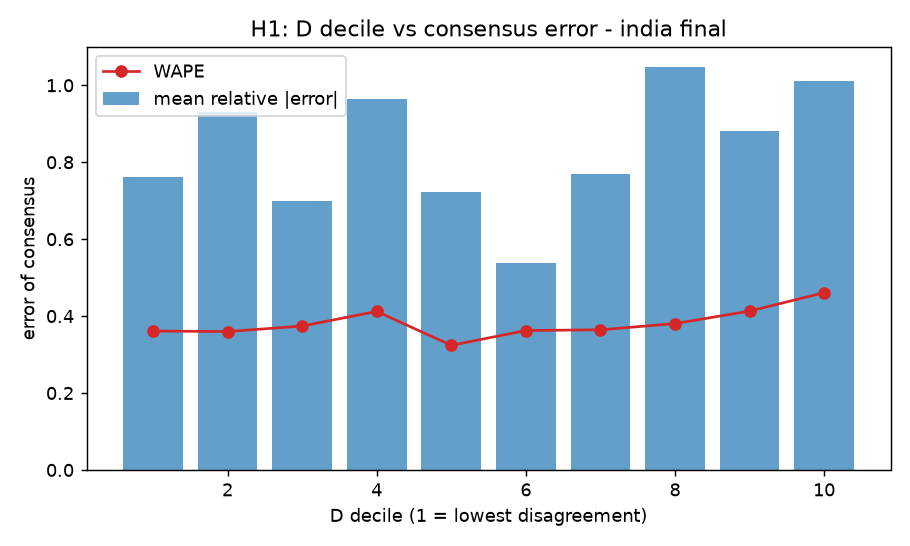
\includegraphics[width=0.49\textwidth]{india_h1_deciles.png}\hfill
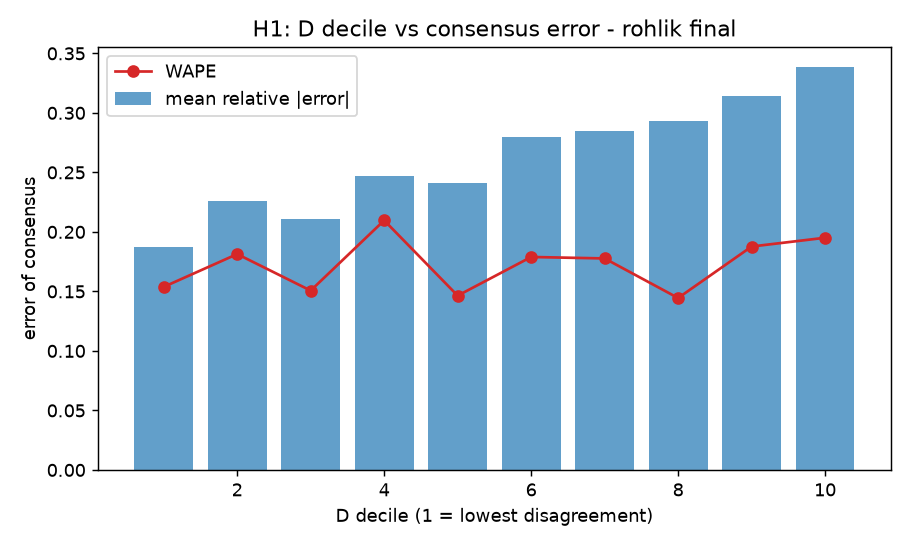
\includegraphics[width=0.49\textwidth]{rohlik_h1_deciles.png}
\caption{Consensus error by decile of disagreement $D$ on the India (left) and Rohlik (right) test
splits. Bars: mean relative absolute error; line: WAPE. The rise with $D$ is weak and non-monotone
on India and clearer on Rohlik.}
\label{fig:deciles}
\end{figure*}

\subsection{H2: The Triggered Cases}
On India, 30.3\% of the 892 triggered test cases improved and 24.6\% worsened (Fig.~\ref{fig:beforeafter}).
With cases clustered by item, the mean gain is 0.027 units [0.003, 0.052] ($p=0.022$, Holm-adjusted
0.044; Wilcoxon treating cases as independent: 0.007). The effect is real but tiny, about 0.2\% of the
mean absolute error, and it did not appear on India validation ($p=0.32$), Rohlik validation
($p=0.26$) or the Rohlik test split (27.6\% improved, 26.6\% worsened, clustered $p=0.59$). Hold
rates of 58.7\% (India) and 53.3\% (Rohlik) show that agents were not simply complying.

\begin{figure}[t]
\centering
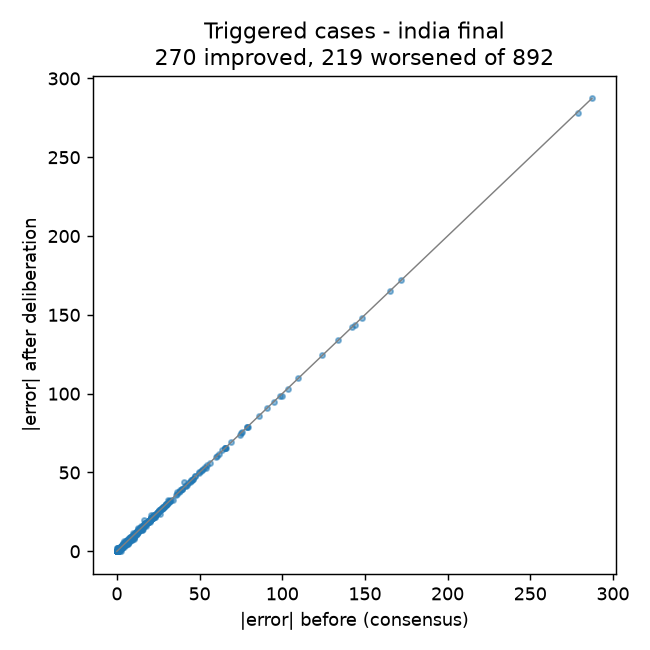
\includegraphics[width=0.85\columnwidth]{india_before_after.png}
\caption{Absolute error before (consensus) and after deliberation for the 892 triggered India test
cases. Nearly all points lie on the diagonal: the bounded revision changes forecasts very little.}
\label{fig:beforeafter}
\end{figure}

\subsection{H3 and H4: Equivalence of the Deliberation Arms}
Table~\ref{tab:equiv} replaces the earlier ``not significant'' statements with equivalence tests.
On India, selective deliberation is equivalent to always-on deliberation, to random triggering and to
no deliberation within 0.5\% of WAPE; on Rohlik, within 1\%. The minimum detectable effects (0.0004
to 0.0022 WAPE, 0.5 to 2.2 seed standard deviations) show that these tests could have detected
differences of 0.1--0.24\% (India) and 0.7--1.3\% (Rohlik) of WAPE. Selective deliberation uses 1,331 rather
than 5,018 LLM calls per 1,000 forecasts on India ($-73\%$) and 696 rather than 4,051 on Rohlik
($-83\%$). H3 is supported; H4 is not (DM $p=0.08$ and $0.57$, Holm-adjusted 0.081 and 1.0), and
the random trigger had the lower WAPE in all three India backtests. Along the cost-accuracy curve
(Fig.~\ref{fig:costacc}), selective triggering stays close to the random band.

\begin{table}[t]
\caption{Equivalence on the Test Splits: $h=1$ WAPE Difference, 90\% Item-Bootstrap CI and Minimum Detectable Effect (80\% Power). Margins Are Relative to the No-Deliberation WAPE (0.3777 India, 0.1746 Rohlik).}
\label{tab:equiv}
\centering
\scriptsize
\setlength{\tabcolsep}{3pt}
\begin{tabular}{@{}lccc@{}}
\toprule
Comparison & Diff [90\% CI] & MDE & Equivalent at \\
\midrule
\multicolumn{4}{@{}l}{\emph{India}} \\
Selective -- always-on & $+0.0002$ [$-0.0003$, $0.0007$] & 0.0008 & 0.5\% \\
Selective -- random    & $-0.0003$ [$-0.0005$, $-0.0000$] & 0.0004 & 0.5\% \\
Always-on -- none      & $-0.0004$ [$-0.0009$, $0.0001$] & 0.0009 & 0.5\% \\
\midrule
\multicolumn{4}{@{}l}{\emph{Rohlik}} \\
Selective -- always-on & $+0.0004$ [$-0.0009$, $0.0016$] & 0.0021 & 1\% \\
Selective -- random    & $-0.0002$ [$-0.0009$, $0.0004$] & 0.0012 & 1\% \\
Always-on -- none      & $-0.0005$ [$-0.0017$, $0.0009$] & 0.0022 & 1\% \\
\bottomrule
\end{tabular}
\end{table}

\begin{figure*}[t]
\centering
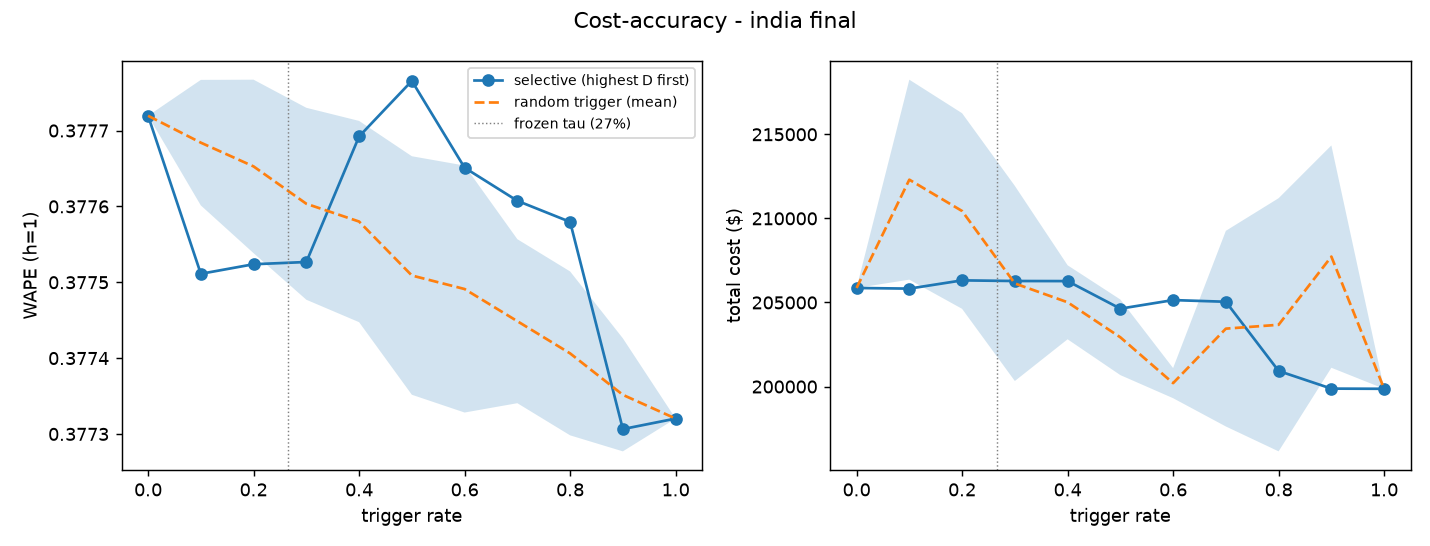
\includegraphics[width=0.49\textwidth]{india_cost_accuracy.png}\hfill
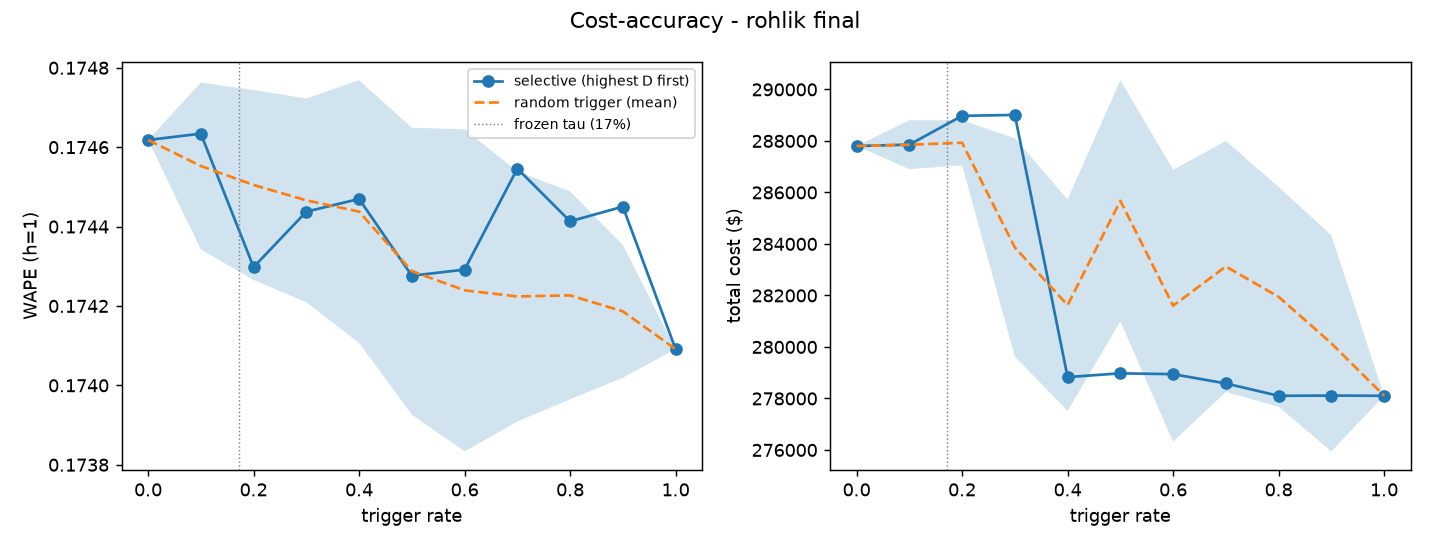
\includegraphics[width=0.49\textwidth]{rohlik_cost_accuracy.png}
\caption{Cost-accuracy curves on the India (left pair) and Rohlik (right pair) test splits: $h=1$
WAPE and total inventory cost as the share of deliberated cases rises from 0 to 1, for selective
triggering (highest $D$ first) and random triggering (mean and band over draws). The dotted line
marks the frozen $\tau$.}
\label{fig:costacc}
\end{figure*}

\subsection{H5: Inventory}
ETS has the lowest India test cost (\$138,621 vs \$206,313 for RetailSense, per-item difference
$+\$1{,}128$ [220, 2,211]) although it is less accurate, because the policy also uses the bands and
lost-sales cost dominates. On Rohlik the all-features LightGBM is cheapest (\$133,467 vs \$287,344).
H5 is not supported. Table~\ref{tab:inventory} reports the inventory outcomes separately from
accuracy, all under the same policy and costs. The multi-agent systems have mid-range stockout and
fill rates. They never trigger REDUCE, and their higher cost comes from lost sales, not from excess
stock. Always-on deliberation is the cheapest multi-agent system on both datasets, but it is not
significantly cheaper than RetailSense (India per-item $+\$107$ [$-6$, 266]). So the data do not
show that the multi-agent design gives better inventory decisions despite its higher WAPE.

\begin{table}[t]
\caption{Test Inventory Outcomes Under One $(s,S)$ Policy. Stockout: Share of Item-Days With Lost
Sales; Fill: Units Sold / Demand (Service Level); Overstock: Mean Units Above the REDUCE Level.}
\label{tab:inventory}
\centering
\scriptsize
\setlength{\tabcolsep}{2.5pt}
\begin{tabular}{@{}l rrrr rrrr@{}}
\toprule
 & \multicolumn{4}{c}{India (simulated)} & \multicolumn{4}{c}{Rohlik (real)} \\
\cmidrule(lr){2-5}\cmidrule(l){6-9}
System & Stockout & Fill & Overst. & Cost (k\$) & Stockout & Fill & Overst. & Cost (k\$) \\
\midrule
Seasonal naive & 1.04\% & 0.989 & 6.48 & 199.8 & 0.80\% & 0.989 & 0.81 & 509.4 \\
ETS & \textbf{0.65\%} & \textbf{0.992} & 2.77 & \textbf{138.6} & \textbf{0.39\%} & 0.996 & 1.73 & 262.9 \\
LightGBM, all feat. & 1.10\% & 0.990 & 0.02 & 183.3 & \textbf{0.39\%} & \textbf{0.999} & 0.00 & \textbf{133.5} \\
Historical agent & 1.22\% & 0.986 & 0.00 & 232.9 & 0.48\% & 0.994 & 0.00 & 314.9 \\
Multi-agent, conf. & 0.86\% & 0.989 & 0.00 & 205.9 & 0.45\% & 0.994 & 0.00 & 287.8 \\
Random trigger & 0.92\% & 0.989 & 0.00 & 206.4 & 0.45\% & 0.994 & 0.00 & 289.3 \\
Always-on & 0.89\% & 0.989 & 0.00 & 199.9 & 0.42\% & 0.995 & 0.00 & 278.1 \\
RetailSense & 0.86\% & 0.989 & 0.00 & 206.3 & 0.45\% & 0.994 & 0.00 & 287.3 \\
\bottomrule
\end{tabular}
\end{table}

\subsection{Case Study}
The highest-$D$ triggered India test case (sevai\_2, d\_1907, $D=0.602$, Fig.~\ref{fig:case}) had a
consensus of 3.35 units against an actual 2.0. The critic described the conflict only in general
terms, and the revisions left the forecast at 3.35.

\begin{figure}[t]
\centering
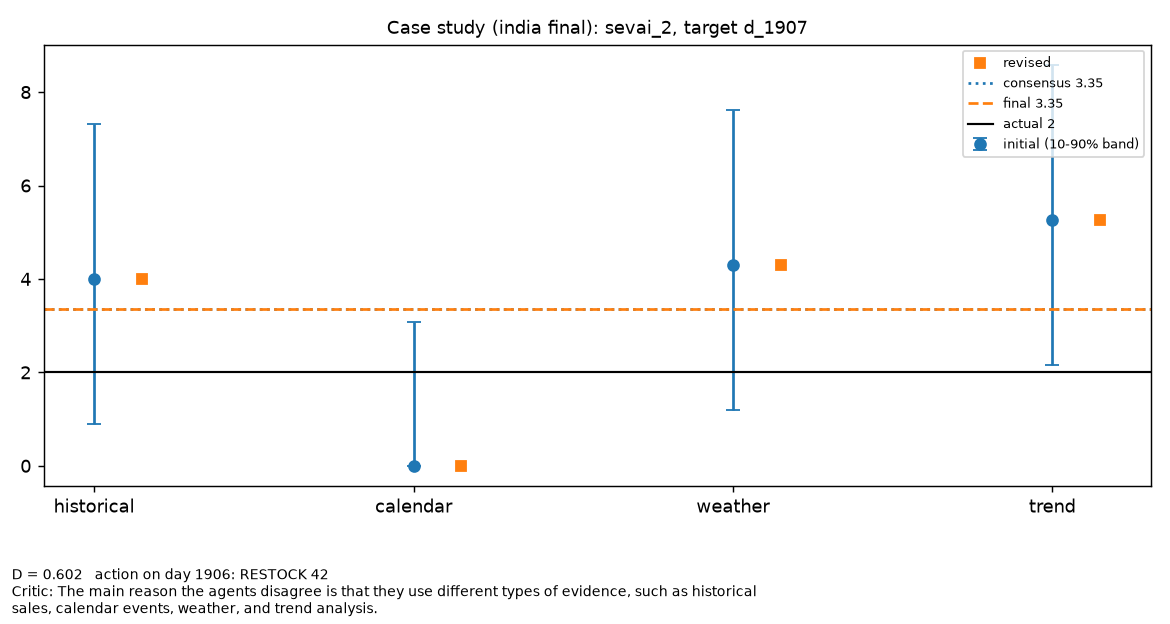
\includegraphics[width=\columnwidth]{india_case_study.png}
\caption{Case study, the highest-$D$ triggered India test case: each agent's initial forecast with its
10--90\% band, its revised value, the consensus and final forecast (both 3.35) and the actual (2).}
\label{fig:case}
\end{figure}

% =====================================================================
\section{Diagnosis: Why Selective Deliberation Fails}\label{sec:diagnosis}

All analyses in this section are post hoc and use validation data
(Section~\ref{sec:setup}-D) except where stored test outputs are named.

\subsection{Is the Weak Signal an Artefact of Correlated Agents?}
The frozen agents fail the planned 0.95 independence gate (pooled forecast correlation 0.986--1.000
on India, 0.994--0.997 on Rohlik), which invites the objection that H1 and H4 were set up to fail.
Two variants test this (Table~\ref{tab:designs}). \emph{Item-aware} agents keep the residual design
but also see item identity. \emph{Independent} agents forecast demand directly from item identity and
their own evidence only, with no sales history and no baseline input; their forecasts are
essentially uncorrelated within each item ($-0.13$ to $0.19$), so their disagreement is between
genuinely independent views. The pooled correlation stays near or above 0.95 even then, because item
identity alone sets each item's level: the gate as defined measures between-item level, not
agreement.

With independent agents, $D$ predicts the error of the \emph{consensus} better on Rohlik ($\rho$
0.099 to 0.239, AUROC 0.570 to 0.667). But that consensus now contains much weaker agents (context
agent WAPE 0.247--0.257 against 0.173--0.176), and $D$ is predicting the error they bring in. As a
warning for large errors of the strong Historical forecast, $D$ adds at most 0.013 AUROC beyond band
width and volume in every design and dataset. Disagreement fails as a risk signal even when the
agents are independent.

\begin{table}[t]
\caption{Agent Designs on Validation. AUROC of Band Width + Volume $\rightarrow$ With $D$ Added, for the Worst 20\% of Consensus Errors and of Historical-Agent Errors}
\label{tab:designs}
\centering
\scriptsize
\setlength{\tabcolsep}{2.5pt}
\begin{tabular}{@{}lccc@{}}
\toprule
 & Residual (frozen) & Item-aware & Independent \\
\midrule
\multicolumn{4}{@{}l}{\emph{India}} \\
Within-item corr.     & 0.76--1.00 & 0.72--0.99 & $-0.04$--0.19 \\
Pooled corr.          & 0.986--1.000 & 0.984--1.000 & 0.962--0.986 \\
Consensus WAPE        & 0.3770 & 0.3751 & 0.3773 \\
H1 $\rho$ / AUROC     & 0.064 / 0.535 & 0.034 / 0.519 & 0.044 / 0.547 \\
Consensus errors      & 0.599$\rightarrow$0.603 & 0.593$\rightarrow$0.595 & 0.584$\rightarrow$0.590 \\
Historical errors     & 0.595$\rightarrow$0.600 & 0.595$\rightarrow$0.597 & 0.587$\rightarrow$0.600 \\
\midrule
\multicolumn{4}{@{}l}{\emph{Rohlik}} \\
Within-item corr.     & 0.90--0.96 & 0.81--0.94 & $-0.13$--0.08 \\
Pooled corr.          & 0.994--0.997 & 0.988--0.996 & 0.946--0.976 \\
Consensus WAPE        & 0.1689 & 0.1684 & 0.1972 \\
H1 $\rho$ / AUROC     & 0.099 / 0.570 & 0.078 / 0.557 & 0.239 / 0.667 \\
Consensus errors      & 0.712$\rightarrow$0.712 & 0.714$\rightarrow$0.714 & 0.722$\rightarrow$0.751 \\
Historical errors     & 0.710$\rightarrow$0.710 & 0.711$\rightarrow$0.712 & 0.711$\rightarrow$0.711 \\
\bottomrule
\end{tabular}
\end{table}

\subsection{Does the Critic Find the Evidence That Mattered?}
Because the simulator logs every demand multiplier, each India case has a known \emph{true driver}:
the context agent whose logged effect (Weather: weather; Calendar: festival and payday; Trend:
interest shock) moves demand most, when it moves demand by at least 10\%. On the 840 test cases with
a driver, the frozen 8B critic rated the driver's agent ``strong'' 18.7\% of the time against 10.4\%
for the other context agents (difference $+8.3$ points [5.2, 11.7]; validation $+4.0$ [$-1.1$, 9.2]).
The critic therefore partly identifies the right evidence. The revisions do not act on it: the
driver's agent received the same weight multiplier as the others ($-0.002$ [$-0.008$, 0.003]) and was
the most up-weighted agent in 31.8\% of cases, against 33.3\% by chance. The failure lies as much in
the step from critique to revision as in the critique itself.

\subsection{Does a Stronger Critic Help?}
Table~\ref{tab:critic} reruns the frozen prompt with Gemma~4 31B on 300 validation cases and replays
Llama~3.1~8B on exactly the same cases from the cache. The larger critic carries its critique into
the revision: on the 59 India cases with a true driver it moves weight toward the driver's agent
($+0.088$ [0.017, 0.153]; the driver's agent is the most up-weighted in 54\% of cases), which the 8B
critic does not ($-0.002$ [$-0.022$, 0.019]; 27\%). Deliberating every case then lowers India WAPE
by 0.9\%, but on Rohlik it does not help, and with either critic selecting cases by $D$ is no better
than selecting them at random. A stronger critic improves deliberation; it does not make $D$ a
useful trigger. One caution: the 31B critic let the Trend agent hold its position in only 3.7\% of
revisions, close to the coercion warning level of the hold-rate gate, while the same prompt gave the
8B critic 57\%.

\begin{table}[t]
\caption{Critic Strength on 300 Validation Cases of the Frozen Agents (Same Cases for Both Critics)}
\label{tab:critic}
\centering
\scriptsize
\setlength{\tabcolsep}{2.5pt}
\begin{tabular}{@{}lcccc@{}}
\toprule
 & \multicolumn{2}{c}{India} & \multicolumn{2}{c}{Rohlik} \\
\cmidrule(lr){2-3}\cmidrule(l){4-5}
 & 8B & 31B & 8B & 31B \\
\midrule
WAPE, no deliberation   & 0.3658 & 0.3658 & 0.1451 & 0.1451 \\
WAPE, always-on         & 0.3655 & 0.3625 & 0.1500 & 0.1457 \\
WAPE, selective         & 0.3662 & 0.3652 & 0.1455 & 0.1454 \\
WAPE, random (sd)       & 0.3658 (.0005) & 0.3650 (.0014) & 0.1465 (.0011) & 0.1454 (.0013) \\
Triggered: improved     & 28\% & 53\% & 33\% & 33\% \\
Triggered: worsened     & 31\% & 45\% & 28\% & 41\% \\
Hold rate               & 53\% & 40\% & 55\% & 70\% \\
\bottomrule
\end{tabular}
\end{table}

\subsection{Independent Agents With the Stronger Critic}
The most favourable combination, independent agents with the 31B critic, produced the only large
deliberation effect in the study: on Rohlik, 64\% of triggered cases improved and 23\% worsened
(Wilcoxon $p<0.001$), always-on deliberation lowered the agents' own consensus WAPE from 0.1736 to
0.1619, and selective triggering (0.1643) beat random triggering (0.1704, sd 0.0033). Scored against
the frozen systems on the same 300 cases, however, this gain is repair: the deliberated forecast is
still significantly worse than the frozen consensus ($+0.0167$ [0.0004, 0.0353]) and the
all-features LightGBM (0.1360). On India the same combination made always-on deliberation worse
(0.3651 to 0.3693; 36\% improved, 59\% worsened). No combination of agent design (residual,
item-aware, independent), critic (8B, 31B) and trigger beat the frozen consensus by a significant
margin, and none beat the single all-features LightGBM.

\subsection{Is the Critic Decorative? Revision Without the Critic}
An ablation removes the critic and keeps everything else (\texttt{val\_nocritic\_300.csv}): on the
same 300 validation cases, each agent sees the other agents' forecasts and evidence instead of a
critic report and gets the same bounded revision round. The prompt was the v1 revision prompt with
only the critic references removed; it was written for this ablation and never used in the study. Without the critic, agents
held their position in 99.4\% (India) and 99.0\% (Rohlik) of revisions, against 53--55\% with it,
and changed the forecast on only 2--3\% of cases. With the critic, always-on deliberation changed
58--60\% of cases but improved about as many as it worsened (India 28\% / 33\%, Rohlik 28\% / 30\%).
Always-on WAPE without minus with the critic was $-0.0001$ [$-0.0023$, 0.0027] on India and
$-0.0051$ [$-0.0108$, 0.0021] on Rohlik, where the critic made always-on worse than no deliberation
(0.1500 vs 0.1451). The critic therefore drives almost all revision activity, but the revisions it
causes do not improve accuracy.

\subsection{Can the Trigger Be Learned?}
A learned trigger modelled the deliberation gain from the signals available before any LLM call
($D$, its range, the Historical band width and volume) with time-blocked cross-validation on the
1,500 stored validation deliberations. It was no better than random at any trigger rate on either
dataset; its score correlated with the realised gain at $\rho=0.023$ (India) and $-0.022$ (Rohlik).
A perfect trigger would have lowered WAPE by about 1\% (India) and 4\% (Rohlik), so the gains exist
but cannot be located in advance from these signals.

Each pre-call signal was also scored alone at the study's 20\% call budget, adding the Historical
agent's trailing 28-day WAPE (\texttt{val\_trigger\_signals.csv}). The signals separate two questions.
As \emph{risk} flags for the worst 20\% of errors, band width (AUROC 0.59 India, 0.73 Rohlik),
volume (0.61, 0.70) and trailing error (0.55, 0.71) all match or beat $D$ (0.55, 0.56). As \emph{benefit}
flags, none predicts where deliberation helps: $|\rho(\text{signal},\text{gain})|\le0.03$ for every
signal, and $\le0.04$ for a learned trigger on all five. None is better than random at the same
budget by even one standard deviation (best: $D$ on India, $z=-0.12$; learned on Rohlik, $z=-0.96$).
Within each triggered set, deliberation improved 26--42\% of cases, worsened 27--40\% and left
18--46\% unchanged. Flagging risky forecasts is therefore a different task from flagging fixable
ones. No signal available before the call meets the bar of beating random triggering on validation,
so none was carried to the test split.

\subsection{Foundation-Model Baseline}
Zero-shot Chronos-Bolt (small)~\cite{ansari2024}, given each item's sales history up to the origin,
reached validation $h=1$ WAPE 0.3708 on India and 0.1642 on Rohlik: statistically tied with the
all-features LightGBM (0.3670 and 0.1620; differences $+0.004$ [$-0.004$, 0.010] and $+0.002$
[$-0.008$, 0.015]) and, without any training on these data, lower in point estimate than the
multi-agent consensus (0.3770 and 0.1689), though that difference is not significant (India
$-0.006$ [$-0.016$, 0.001], DM $p=0.07$; Rohlik $-0.005$ [$-0.012$, 0.002], $p=0.26$). Chronos was
evaluated on validation only and is not part of the locked test comparison.

% =====================================================================
\section{Discussion}\label{sec:discussion}

\subsection{Why Disagreement Is a Weak Trigger}
Disagreement is known to be only a partial proxy for uncertainty~\cite{zarnowitz1987,whitaker1998}.
This study adds three mechanisms. First, when agents share a baseline, $D$ measures the size of small
adjustments. Second, when agents are made independent, the evidence that is not in the sales history
is too weak to stand alone, so $D$ grows with the errors of the weak agents rather than with the risk
of the forecast that matters. Third, the large errors of a good forecaster are already predicted by
its own band width and the item's volume. Disagreement adds little in all three cases.

\subsection{Why Deliberation Helps Little}
Self-critique without reliable external feedback often fails~\cite{huang2024}, and the ground-truth
analysis shows where: an 8B critic partly names the right evidence but its revisions do not move
weight toward it. A 31B critic closes that gap and helps a little when it sees every case, which
suggests that critic quality limits the gain from deliberation, while the trigger limits the gain
from selectivity. Since RetailSense keeps the LLM away from the demand number~\cite{gruver2023,jin2024},
even a good critic can only re-weight forecasts that are already similar, consistent with evidence that
LLM components add little to numeric forecasting~\cite{tan2024}.

\subsection{Accuracy and Inventory Cost}
The cost ranking differs from the accuracy ranking because the $(s,S)$ policy uses the bands and
lost-sales cost dominates~\cite{silver2017}, in line with earlier
work~\cite{syntetos2010,kourentzes2020}. Evaluating forecasts through a common simulator is
therefore necessary.

\subsection{Practical Implications}
A practitioner who wants an LLM in the forecasting loop should not expect agent disagreement to
decide when to call it. Selective calling does save 73--83\% of the calls at no measurable accuracy
cost, but only because deliberation itself changes little; a strong single model or a zero-shot
foundation model is the better default here. Selective deliberation needs a trigger that predicts
where deliberation \emph{helps}, not where forecasts look risky, and, on this evidence, inputs from
the critic itself rather than from the agents' forecasts.

\subsection{Threats to Validity}\label{sec:threats}
\emph{Simulated India sales:} India results describe method behaviour, not a real store; Rohlik
agrees on every hypothesis except H2. \emph{Post-hoc diagnosis:} Section~\ref{sec:diagnosis} was
designed after the test runs; it uses validation data, its deliberation samples are small (300
cases; 59 India cases with a true driver for the critic comparison), and the equivalence margins were
fixed after the test run, which is why three are reported. \emph{Critics:} only two LLMs were tested,
and the 31B critic received the output schema as text rather than through constrained decoding.
\emph{Seeds:} the frozen runs used one LightGBM seed; four further seeds of systems 1--6 on
validation gave a WAPE seed standard deviation (0.0004--0.0006 India) as large as the gaps among
systems 5--9, and left the all-features LightGBM ahead under every seed,
but the LLM arms (systems 7--9) were not rerun under other seeds: a new seed changes every agent
forecast and so every LLM input, which would need a new full set of deliberation calls per seed.
Their variability is bounded only by the random-trigger draws and the item bootstrap. \emph{Signals:} the India interest index is
generated and built to lead demand, and the India validation window has no rainy days and no major
festival. \emph{Censored demand:} sales are capped on stock-out days (1.2\% of India and 5.0\% of
Rohlik test item-days); excluding them changes $h=1$ WAPE by at most 0.016 and leaves the ranking of
systems 1--6 unchanged. \emph{Inventory parameters:} $z=1.65$ is not cost-optimal, but a 0.99 service
level lowers every India cost by 26--33\% and ETS remains cheapest. \emph{Process:} the go/pivot
decision after the early H1 smoke test ($\rho=0.064<0.15$) was recorded retrospectively.

% =====================================================================
\section{Conclusion}\label{sec:conclusion}

RetailSense was evaluated under a frozen protocol on a simulated Indian kirana store with logged
demand drivers and on real Rohlik sales. Table~\ref{tab:hyp} summarises the hypotheses. A single
all-features LightGBM and ETS were the most accurate systems, and a zero-shot foundation model came
close to the best.

\begin{table}[t]
\caption{Hypotheses on the Two Test Splits (Holm-Adjusted Where Tested)}
\label{tab:hyp}
\centering
\footnotesize
\begin{tabularx}{\columnwidth}{@{}lXX@{}}
\toprule
 & India (simulated) & Rohlik (real) \\
\midrule
H1 & Weak: $\rho=0.072$, AUROC 0.539 & Weak: $\rho=0.119$, AUROC 0.579 \\
H2 & Tiny: gain 0.027 units, $p_{\mathrm{adj}}=0.044$; not on validation & Not supported \\
H3 & Equivalent within 0.5\%, $-73\%$ calls & Equivalent within 1\%, $-83\%$ calls \\
H4 & Not supported; equivalent to random & Not supported; equivalent to random \\
H5 & Not supported: ETS cheapest & Not supported: LightGBM cheapest \\
\bottomrule
\end{tabularx}
\end{table}

The main lesson is that disagreement between forecasting agents did not tell an LLM when to
deliberate, and the post-hoc diagnosis rules out the obvious explanations one by one. Correlated
agents are not the whole story, because independent agents do not make $D$ a better warning. A weak
critic is not the whole story, because a stronger critic that acts on the right evidence still gains
nothing from selection by $D$. And the trigger cannot be learned from the signals available before
the LLM is called. Future work should therefore (i)~give a router inputs from a cheap first critic
pass rather than from the forecasts, (ii)~test stronger critics with constrained output across
several seeds, (iii)~build context agents on evidence strong enough to stand alone, and
(iv)~replicate on further real datasets.

% =====================================================================
\begin{thebibliography}{28}

\bibitem{ke2017}
G.~Ke, Q.~Meng, T.~Finley, T.~Wang, W.~Chen, W.~Ma, Q.~Ye, and T.-Y. Liu, ``LightGBM: A highly
efficient gradient boosting decision tree,'' in \emph{Proc. Adv. Neural Inf. Process. Syst.
(NIPS)}, vol.~30, Long Beach, CA, USA, 2017, pp. 3146--3154.

\bibitem{makridakis2022}
S.~Makridakis, E.~Spiliotis, and V.~Assimakopoulos, ``M5 accuracy competition: Results, findings,
and conclusions,'' \emph{Int. J. Forecast.}, vol.~38, no.~4, pp. 1346--1364, 2022,
doi: 10.1016/j.ijforecast.2021.11.013.

\bibitem{du2024}
Y.~Du, S.~Li, A.~Torralba, J.~B. Tenenbaum, and I.~Mordatch, ``Improving factuality and reasoning
in language models through multiagent debate,'' in \emph{Proc. 41st Int. Conf. Mach. Learn.
(ICML)}, Vienna, Austria, 2024, PMLR vol.~235, pp. 11733--11763.

\bibitem{tan2024}
M.~Tan, M.~A. Merrill, V.~Gupta, T.~Althoff, and T.~Hartvigsen, ``Are language models actually
useful for time series forecasting?'' in \emph{Proc. Adv. Neural Inf. Process. Syst. (NeurIPS)},
vol.~37, Vancouver, BC, Canada, 2024.

\bibitem{yang2025}
Y.~Yang, M.~Wang, J.~Wang, P.~Li, and M.~Zhou, ``Multi-agent deep reinforcement learning for
integrated demand forecasting and inventory optimization in sensor-enabled retail supply chains,''
\emph{Sensors}, vol.~25, no.~8, Art. no. 2428, 2025, doi: 10.3390/s25082428.

\bibitem{bates1969}
J.~M. Bates and C.~W.~J. Granger, ``The combination of forecasts,'' \emph{Oper. Res. Q.}, vol.~20,
no.~4, pp. 451--468, 1969, doi: 10.1057/jors.1969.103.

\bibitem{timmermann2006}
A.~Timmermann, ``Forecast combinations,'' in \emph{Handbook of Economic Forecasting}, vol.~1,
G.~Elliott, C.~W.~J. Granger, and A.~Timmermann, Eds. Amsterdam, The Netherlands: Elsevier, 2006,
pp. 135--196.

\bibitem{wang2023}
X.~Wang, R.~J. Hyndman, F.~Li, and Y.~Kang, ``Forecast combinations: An over 50-year review,''
\emph{Int. J. Forecast.}, vol.~39, no.~4, pp. 1518--1547, 2023,
doi: 10.1016/j.ijforecast.2022.11.005.

\bibitem{zarnowitz1987}
V.~Zarnowitz and L.~A. Lambros, ``Consensus and uncertainty in economic prediction,'' \emph{J.
Polit. Econ.}, vol.~95, no.~3, pp. 591--621, 1987, doi: 10.1086/261473.

\bibitem{whitaker1998}
J.~S. Whitaker and A.~F. Loughe, ``The relationship between ensemble spread and ensemble mean
skill,'' \emph{Mon. Weather Rev.}, vol.~126, no.~12, pp. 3292--3302, 1998,
doi: 10.1175/1520-0493(1998)126<3292:TRBESA>2.0.CO;2.

\bibitem{madaan2023}
A.~Madaan \emph{et al.}, ``Self-Refine: Iterative refinement with self-feedback,'' in \emph{Proc.
Adv. Neural Inf. Process. Syst. (NeurIPS)}, vol.~36, New Orleans, LA, USA, 2023.

\bibitem{chen2023}
L.~Chen, M.~Zaharia, and J.~Zou, ``FrugalGPT: How to use large language models while reducing cost
and improving performance,'' arXiv preprint arXiv:2305.05176, May 2023.

\bibitem{ong2025}
I.~Ong \emph{et al.}, ``RouteLLM: Learning to route LLMs from preference data,'' in \emph{Proc.
Int. Conf. Learn. Represent. (ICLR)}, Singapore, 2025.

\bibitem{gruver2023}
N.~Gruver, M.~Finzi, S.~Qiu, and A.~G. Wilson, ``Large language models are zero-shot time series
forecasters,'' in \emph{Proc. Adv. Neural Inf. Process. Syst. (NeurIPS)}, vol.~36, New Orleans, LA,
USA, 2023.

\bibitem{jin2024}
M.~Jin \emph{et al.}, ``Time-LLM: Time series forecasting by reprogramming large language
models,'' in \emph{Proc. Int. Conf. Learn. Represent. (ICLR)}, Vienna, Austria, 2024.

\bibitem{silver2017}
E.~A. Silver, D.~F. Pyke, and D.~J. Thomas, \emph{Inventory and Production Management in Supply
Chains}, 4th~ed. Boca Raton, FL, USA: CRC Press, 2017.

\bibitem{schuirmann1987}
D.~J. Schuirmann, ``A comparison of the two one-sided tests procedure and the power approach for
assessing the equivalence of average bioavailability,'' \emph{J. Pharmacokinet. Biopharm.},
vol.~15, no.~6, pp. 657--680, 1987, doi: 10.1007/BF01068419.

\bibitem{openmeteo}
P.~Zippenfenig, ``Open-Meteo.com Weather API,'' Zenodo, 2023. [Software]. doi:
10.5281/zenodo.7970649.

\bibitem{rohlik}
Rohlik Group. ``Rohlik sales forecasting challenge v2.'' Kaggle.
\url{https://www.kaggle.com/competitions/rohlik-sales-forecasting-challenge-v2} (accessed Oct.~12,
2026).

\bibitem{ansari2024}
A.~F. Ansari \emph{et al.}, ``Chronos: Learning the language of time series,'' \emph{Trans. Mach.
Learn. Res.}, 2024.

\bibitem{huang2024}
J.~Huang \emph{et al.}, ``Large language models cannot self-correct reasoning yet,'' in
\emph{Proc. Int. Conf. Learn. Represent. (ICLR)}, Vienna, Austria, 2024.

\bibitem{sharma2024}
M.~Sharma \emph{et al.}, ``Towards understanding sycophancy in language models,'' in \emph{Proc.
Int. Conf. Learn. Represent. (ICLR)}, Vienna, Austria, 2024.

\bibitem{syntetos2010}
A.~A. Syntetos, K.~Nikolopoulos, and J.~E. Boylan, ``Judging the judges through
accuracy-implication metrics: The case of inventory forecasting,'' \emph{Int. J. Forecast.},
vol.~26, no.~1, pp. 134--143, 2010, doi: 10.1016/j.ijforecast.2009.05.016.

\bibitem{kourentzes2020}
N.~Kourentzes, J.~R. Trapero, and D.~K. Barrow, ``Optimising forecasting models for inventory
planning,'' \emph{Int. J. Prod. Econ.}, vol.~225, Art. no. 107597, 2020,
doi: 10.1016/j.ijpe.2019.107597.

\bibitem{llama3}
A.~Grattafiori \emph{et al.}, ``The Llama 3 herd of models,'' arXiv preprint arXiv:2407.21783,
Jul. 2024.

\bibitem{diebold1995}
F.~X. Diebold and R.~S. Mariano, ``Comparing predictive accuracy,'' \emph{J. Bus. Econ. Stat.},
vol.~13, no.~3, pp. 253--263, 1995.

\bibitem{holm1979}
S.~Holm, ``A simple sequentially rejective multiple test procedure,'' \emph{Scand. J. Stat.},
vol.~6, no.~2, pp. 65--70, 1979.

\end{thebibliography}

\end{document}
